\documentclass{beamer}
\usepackage{tikz}

% internal parameters
\usetheme{Copenhagen}
\usecolortheme{default}
\setbeamertemplate{caption}[numbered]

% packages
\usepackage{graphics}
\usepackage{amsmath}
\usepackage{xcolor}
\usepackage{physics}
\usepackage{fontawesome}
\usepackage{mathrsfs}  
\usepackage{multirow}


\title[Wobbling Motion, NSP-2022]{Evaluation of the Wobbling Motion in Even-Even Nuclei Within a Simple Rotor Model}
\author[Robert, POENARU]{Robert POENARU\inst{1,2}}

\institute[VFU]
{
  \inst{1}%
  Doctoral School of Physics @ UB\\
  Bucharest, Romania
  \and
  \inst{2}%
  Dept. of Th. Phys. @ IFIN-HH\\
  Magurele, Romania
}

\date{\textit{International Conference on Nuclear Structure Properties}\\\textit{\today}}


\expandafter\def\expandafter\insertshorttitle\expandafter{%
  \insertshorttitle\hfill%
  \insertframenumber\,/\,\inserttotalframenumber}
%------------------------------------------------------------
\begin{document}
%---------------------------------------------------------
\frame{\titlepage}
\begin{frame}
  \frametitle{Table of Contents}
\end{frame}

\begin{frame}{Nuclear Deformation}
  \begin{itemize}
    \item Most of the nuclei are either \emph{spherical} or \emph{axially symmetric} in their ground-state.
    \item Deformation parameter $\beta$ (\textit{Bohr, 1969}): preserves axial symmetry
  \end{itemize}
  \begin{figure}
    \centering
    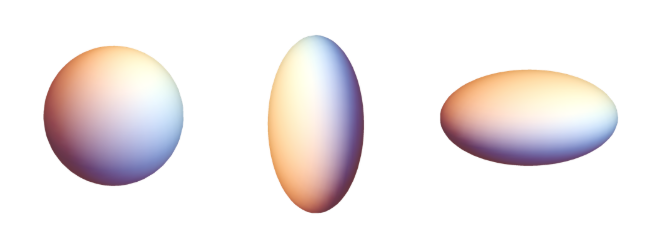
\includegraphics[width=0.99\textwidth]{Figs/nuclear_shapes.png}
    \caption{\textbf{spherical:} $\beta=0$\ \textbf{prolate:} $\beta>0$\ \textbf{oblate:} $\beta<0$}
  \end{figure}
\end{frame}

\begin{frame}
  \frametitle{Nuclear Triaxiality}
  \begin{alertblock}{Non-axial shapes}
    \begin{itemize}
      \item Deviations from symmetric shapes can occur across the chart of nuclides $\to$ \textbf{triaxial nuclei}.
      \item The triaxiality parameter $\gamma$ (\textit{Bohr, 1969}): departure from axial symmetry
    \end{itemize}
  \end{alertblock}
  \begin{figure}
    \centering
    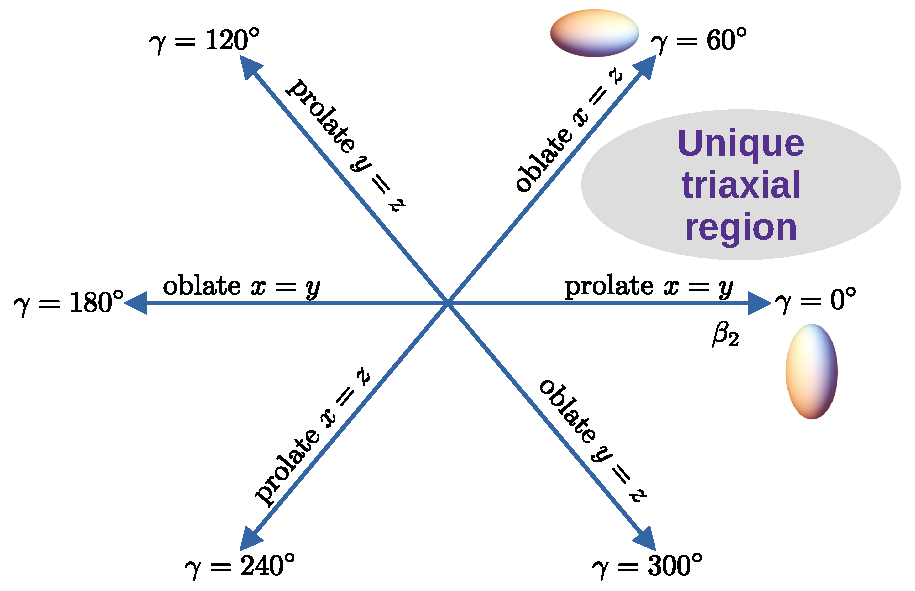
\includegraphics[scale=0.42]{Figs/nice_diagram.pdf}
    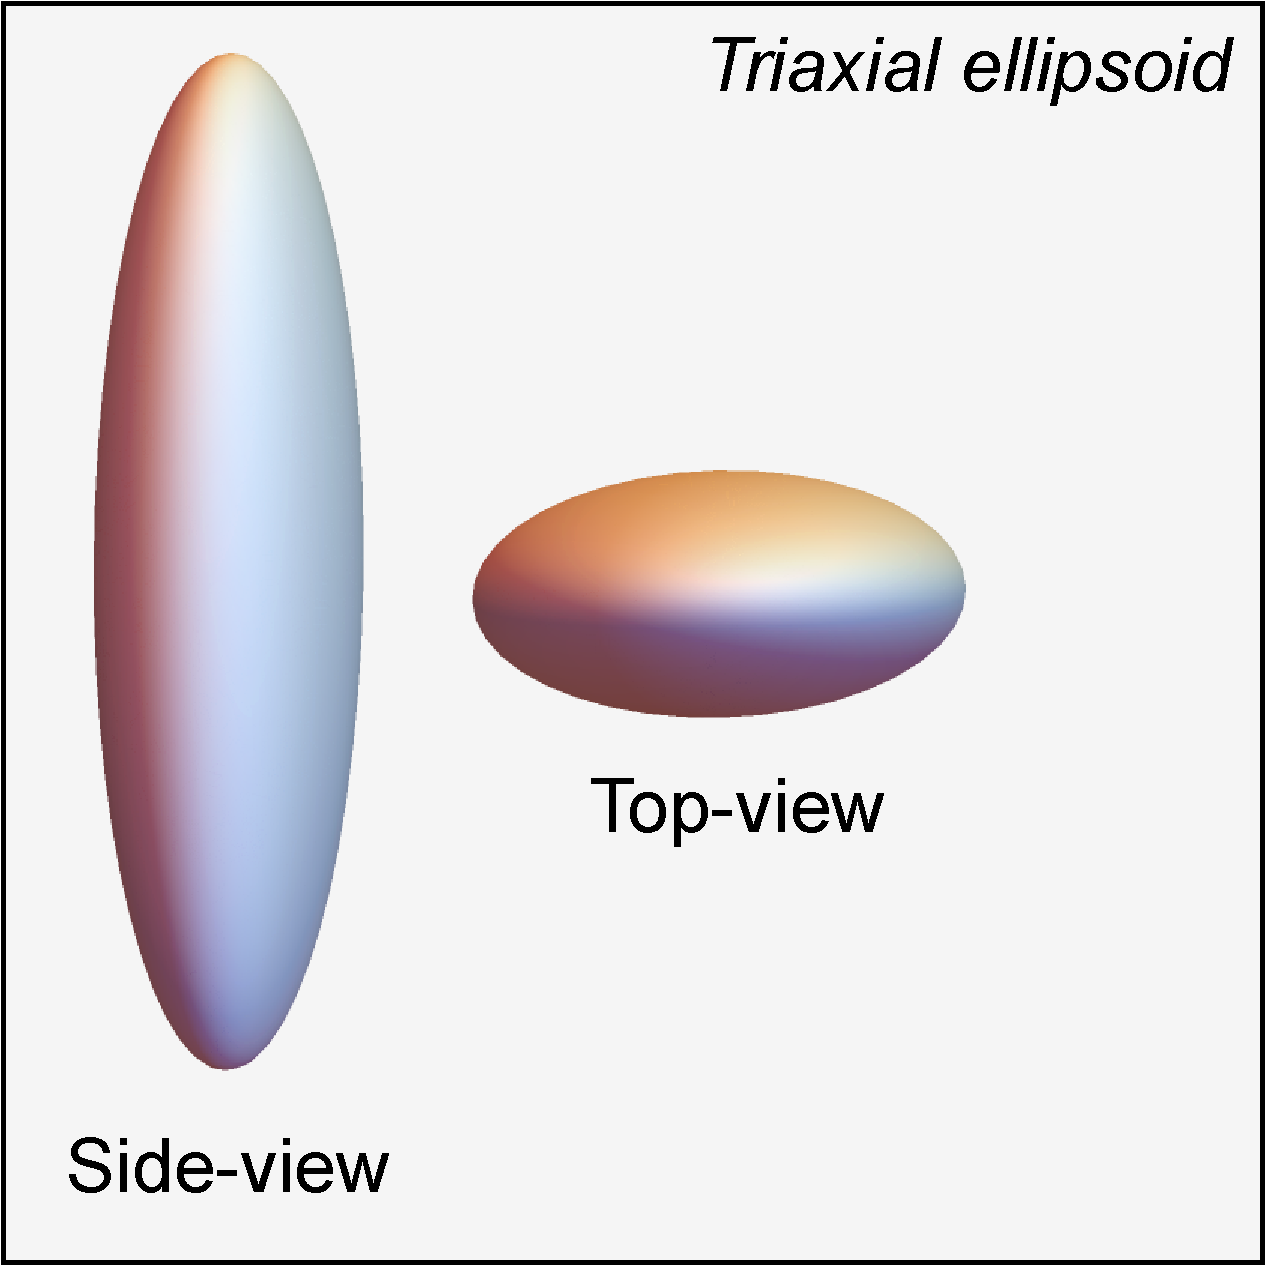
\includegraphics[scale=0.19]{Figs/triaxial-shape.pdf}
    % \caption{The $(\beta,\gamma)$ plane divided into six equivalent parts, depicting nuclear surfaces.}
  \end{figure}
\end{frame}

\begin{frame}
  \frametitle{Fingerprints for Triaxiality}
  \begin{itemize}
    \item Stable triaxial nuclei represent a real challenge for experimentalists and theoreticians
    \item Clear signatures for confirming stable triaxiality in nuclei
    \begin{enumerate}
      \item Chiral symmetry breaking (\textit{Frauendorf, 1997})
      \item \textbf{Wobbling motion} (\textit{Bohr \& Mottelson, 1975})
    \end{enumerate}
  \end{itemize}
  \begin{block}{Wobbling Motion (WM)}
    \begin{itemize}
      \item Unique to non-axial nuclei
      \item Predicted 50 years ago for even-$A$ nuclei (i.e., the simple wobbler)
      \item First experimental evidence for $^{163}$Lu (\textit{Ødegård}, 2001)
      \item Currently confirmed wobblers $A\approx[100,130,160,180]$.
    \end{itemize}
  \end{block}
\end{frame}

\begin{frame}
  \frametitle{Triaxial Rotor Energy}
  \begin{itemize}
    \item Rigid body rotational energy: $E_\text{rot}\propto\frac{\hbar^2}{2\mathcal{J}_\text{max}}I(I+1 )$
    \item A triaxial nucleus can rotate about any of the three axes $\rightarrow$ \emph{rich energy specra spectra}
    % \item Rotation about the axis with \textbf{the largest moment of inertia} (MOI) is energetically the most favorable: 
    \item MOI anisotropy $\rightarrow$ the \emph{main rotation} around $\mathcal{J}_\text{max}$ is disturbed by the other two axes  $\rightarrow$ \textbf{resulting motion of the rotating nucleus has an oscillating behavior}
  \end{itemize}
  \begin{figure}
    \centering
    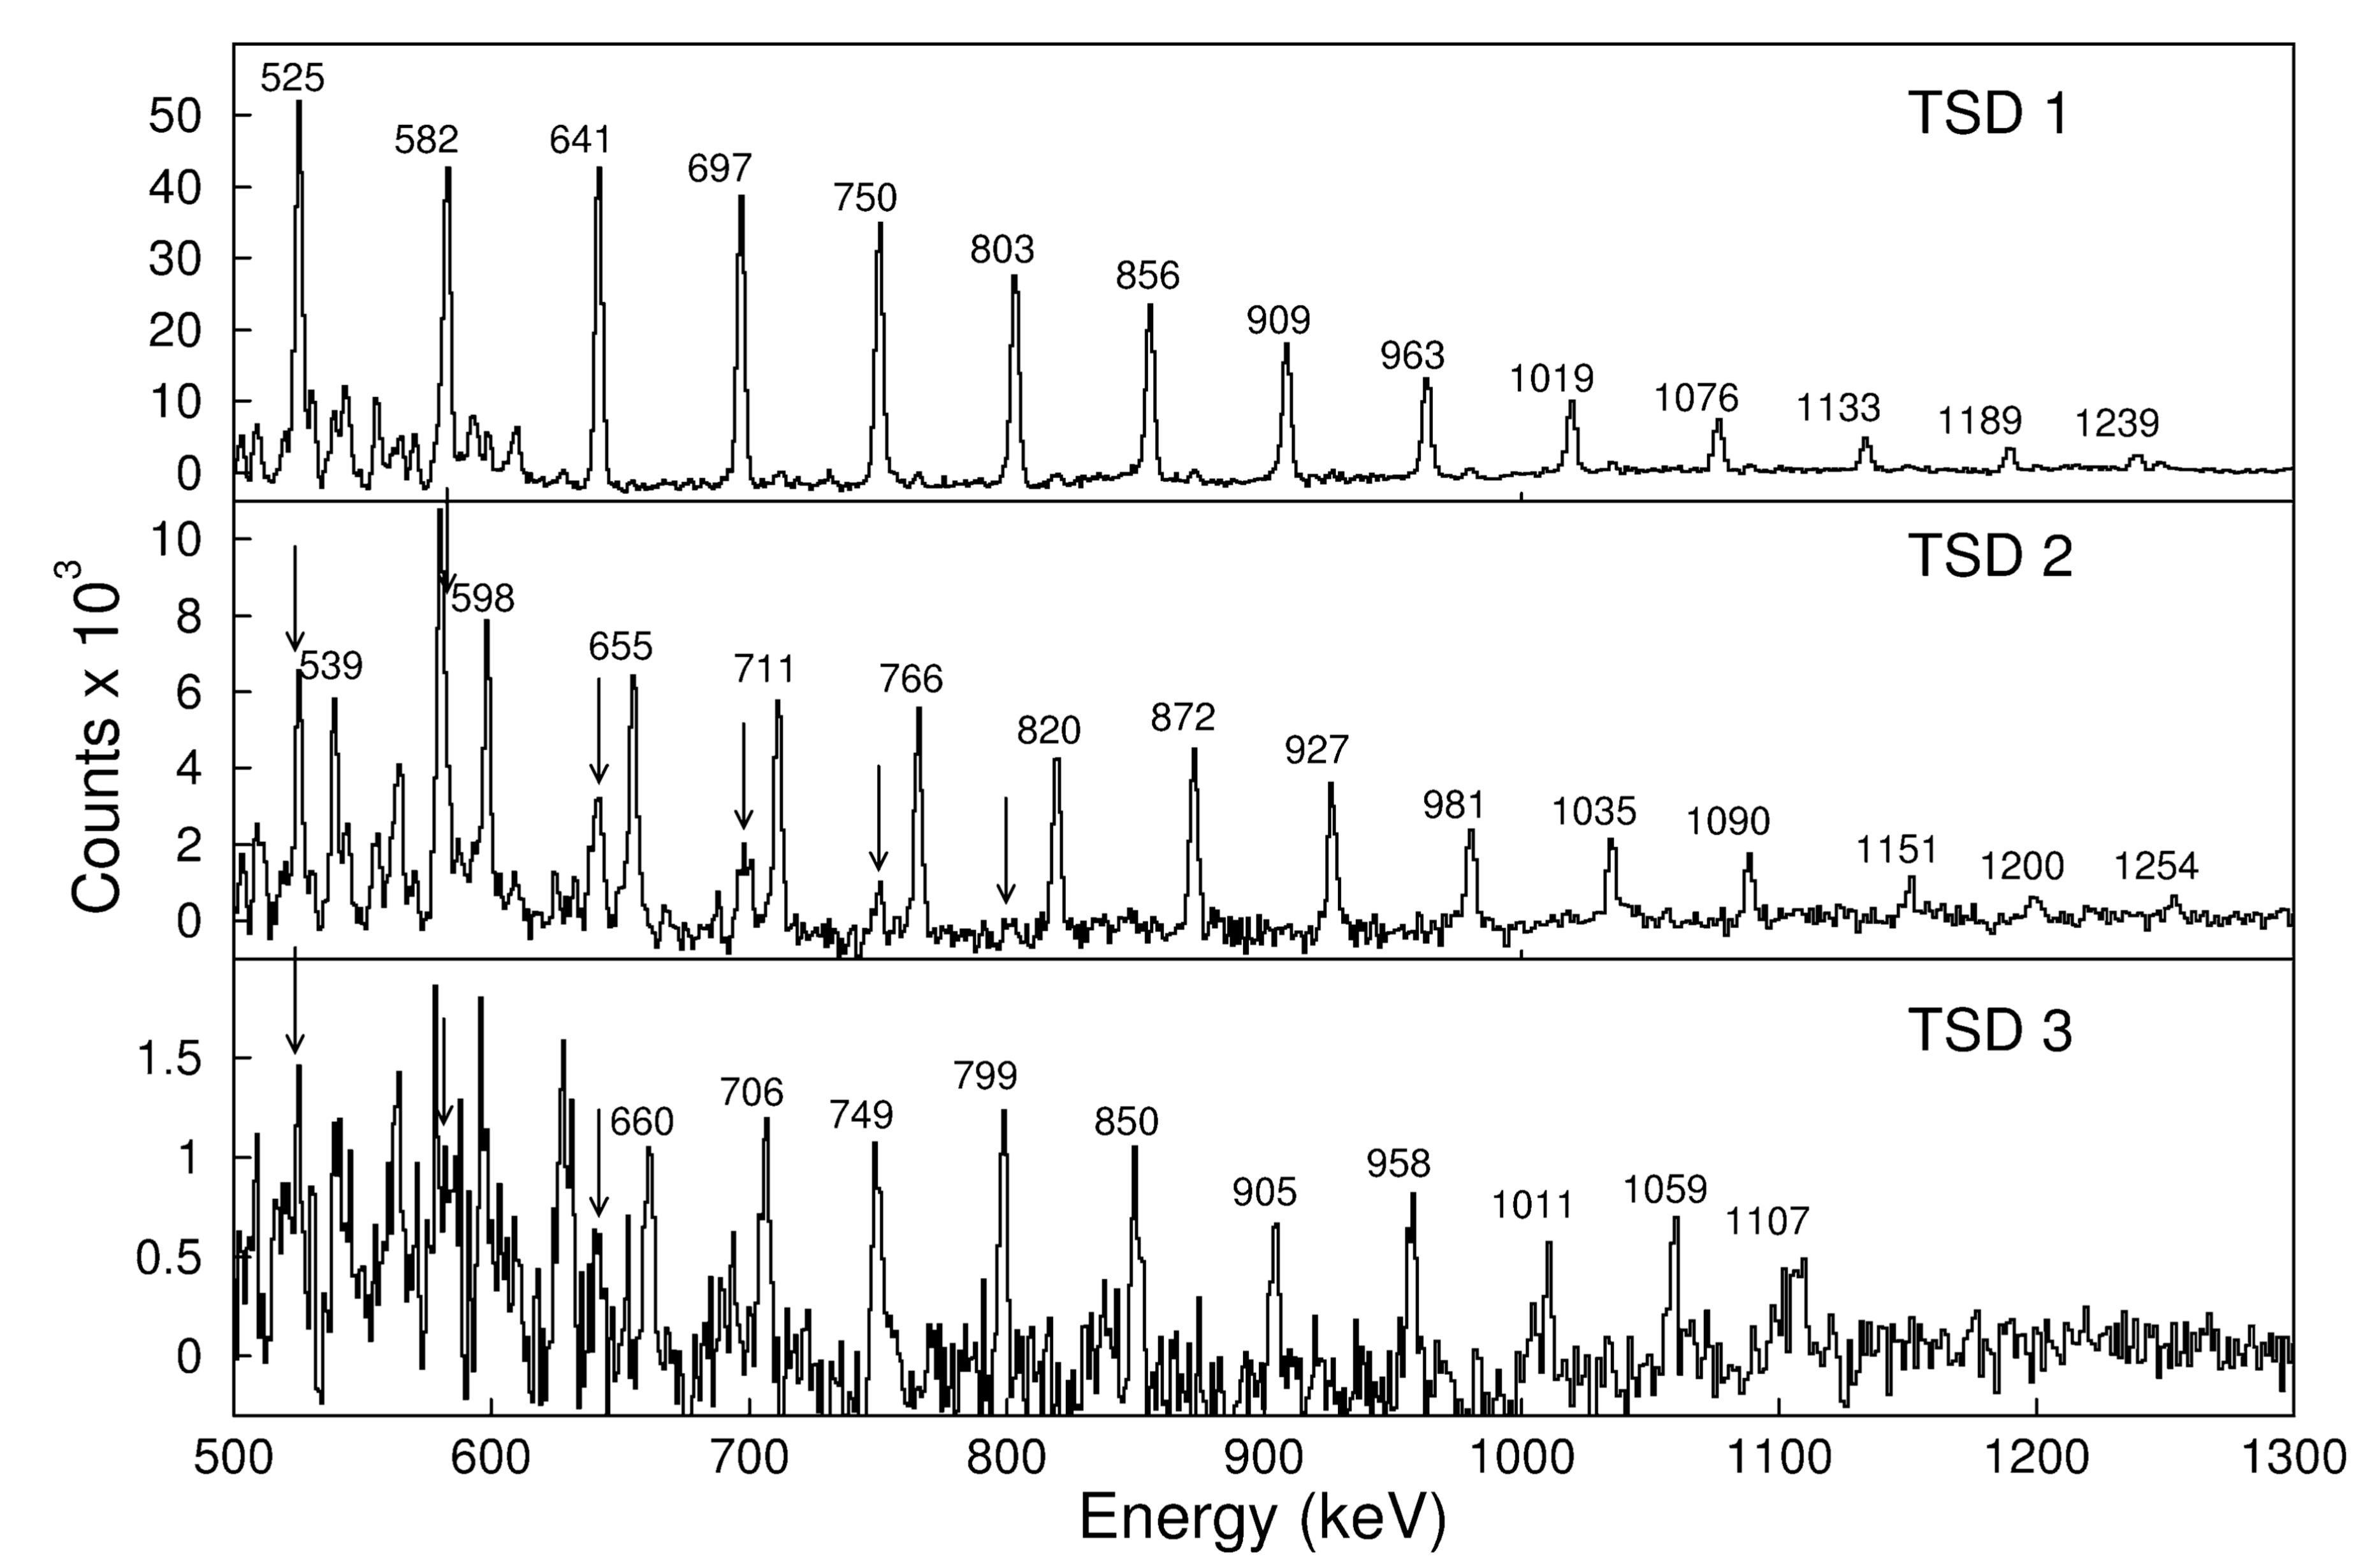
\includegraphics[scale=0.10]{Figs/collective-spectra.pdf}
    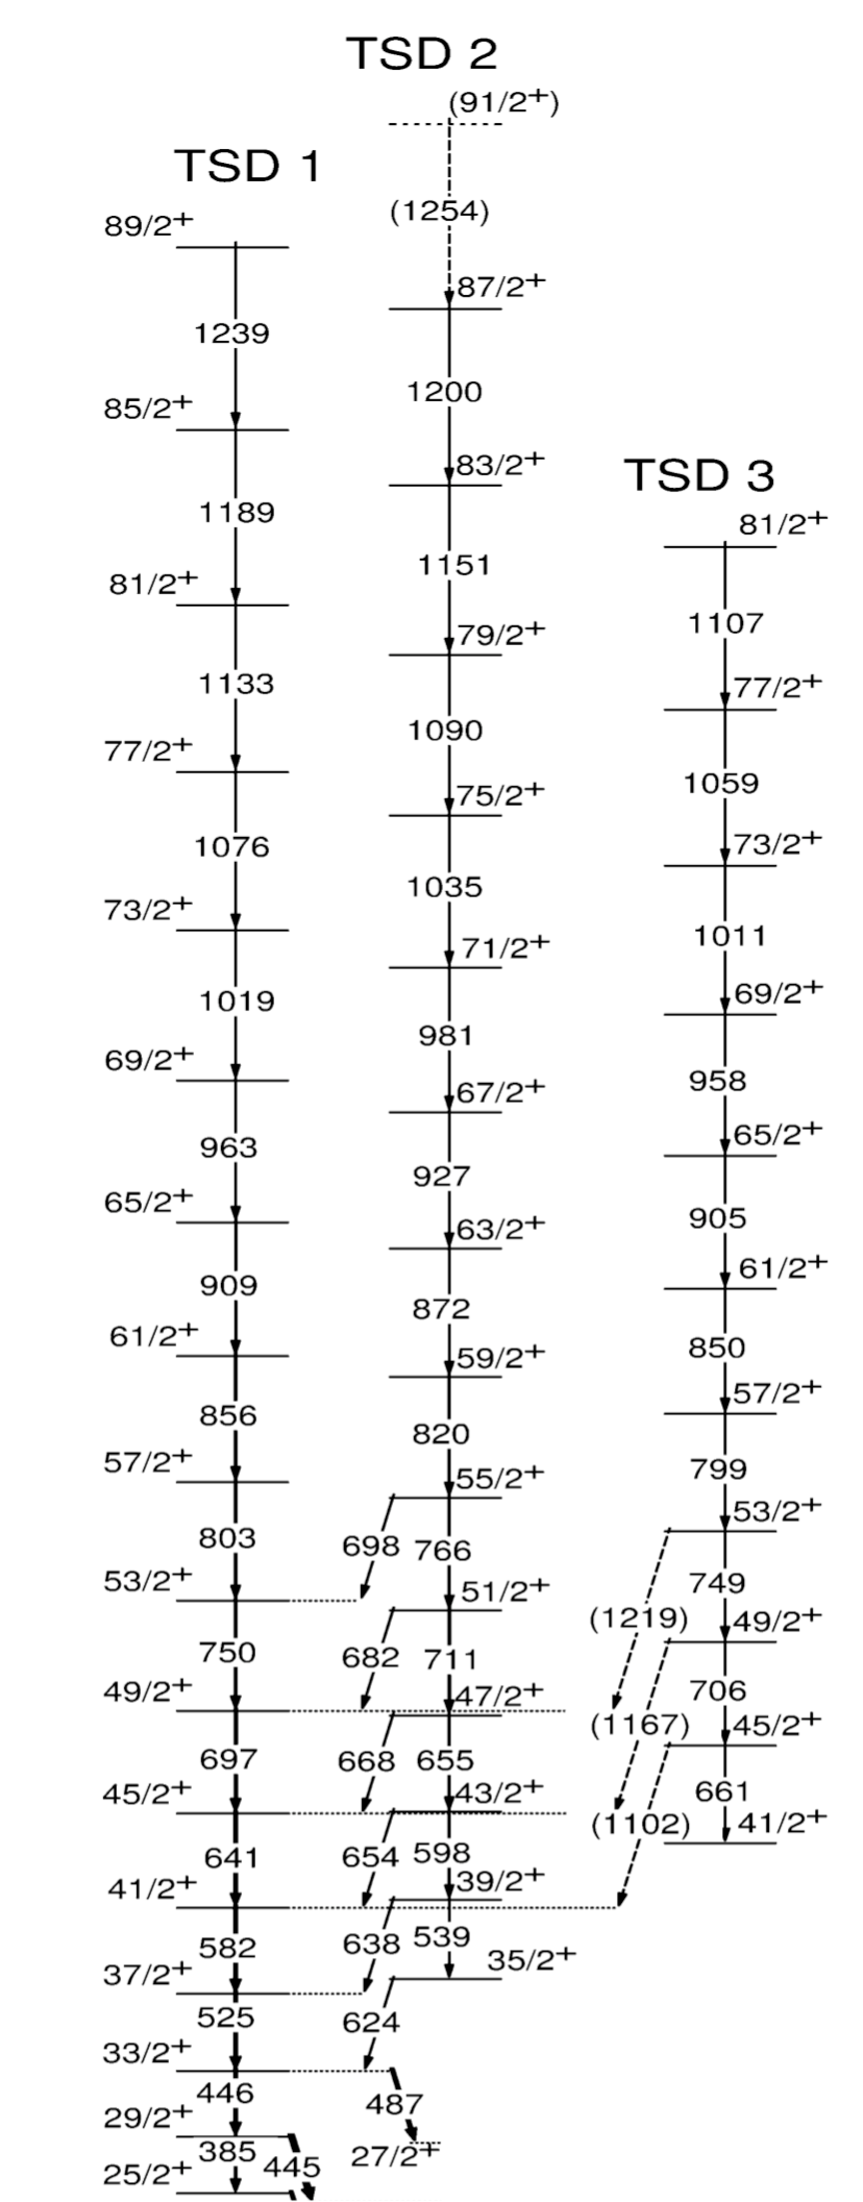
\includegraphics[scale=0.11]{Figs/collective-levels.pdf}
  \end{figure}
  \tiny{\textit{Figures from Schönwaßer et al., 2001}}
\end{frame}

\begin{frame}
  \frametitle{Wobbling Motion}
\begin{itemize}
  \item Oscillatory character of $\mathbf{I}$ $\rightarrow$ $\mathbf{I}$ \emph{disaligned} w.r.t. body-fixed axes
  \item The a.m. \textbf{precesses} and \textbf{wobbles} around the axis with $\mathcal{J}_\text{max}$
  \item The precession of $\mathbf{I}$ can increase by \textbf{tilting} 
  \item Tilting by an energy quanta $\sim$ \emph{vibrational character} $\rightarrow$ \textbf{wobbling phonon} $n_w=0,1,2...$
\end{itemize}
  \begin{figure}
    \centering
    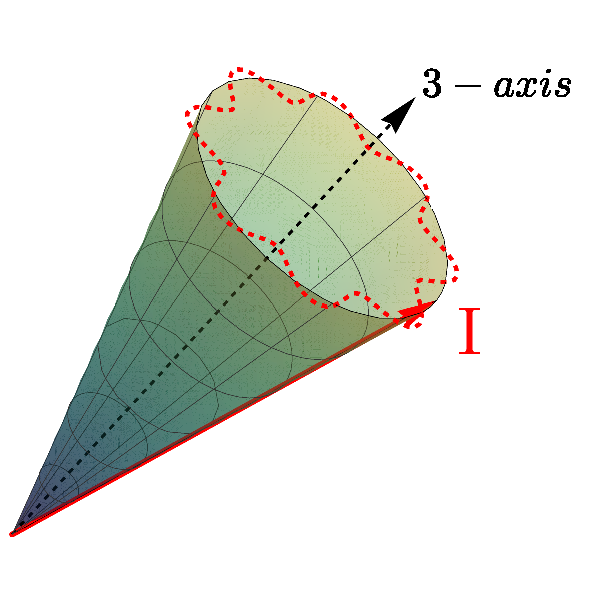
\includegraphics[scale=0.39]{Figs/precessional_cone_2.pdf}
    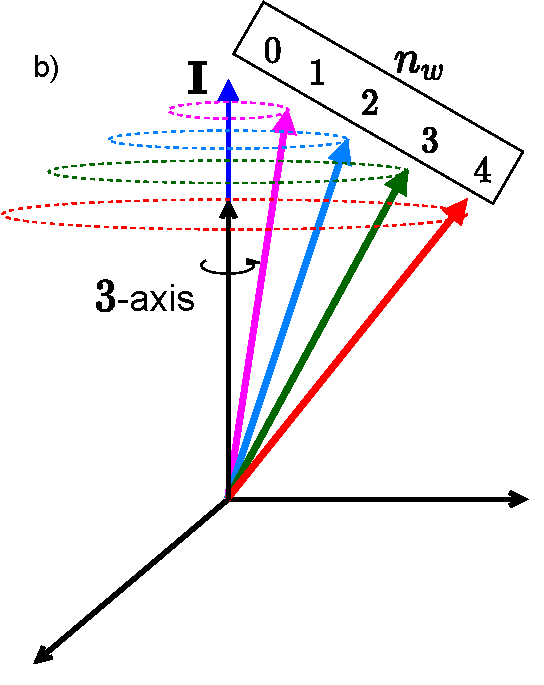
\includegraphics[scale=0.32]{Figs/wobbling_n_schematic-2.pdf}
    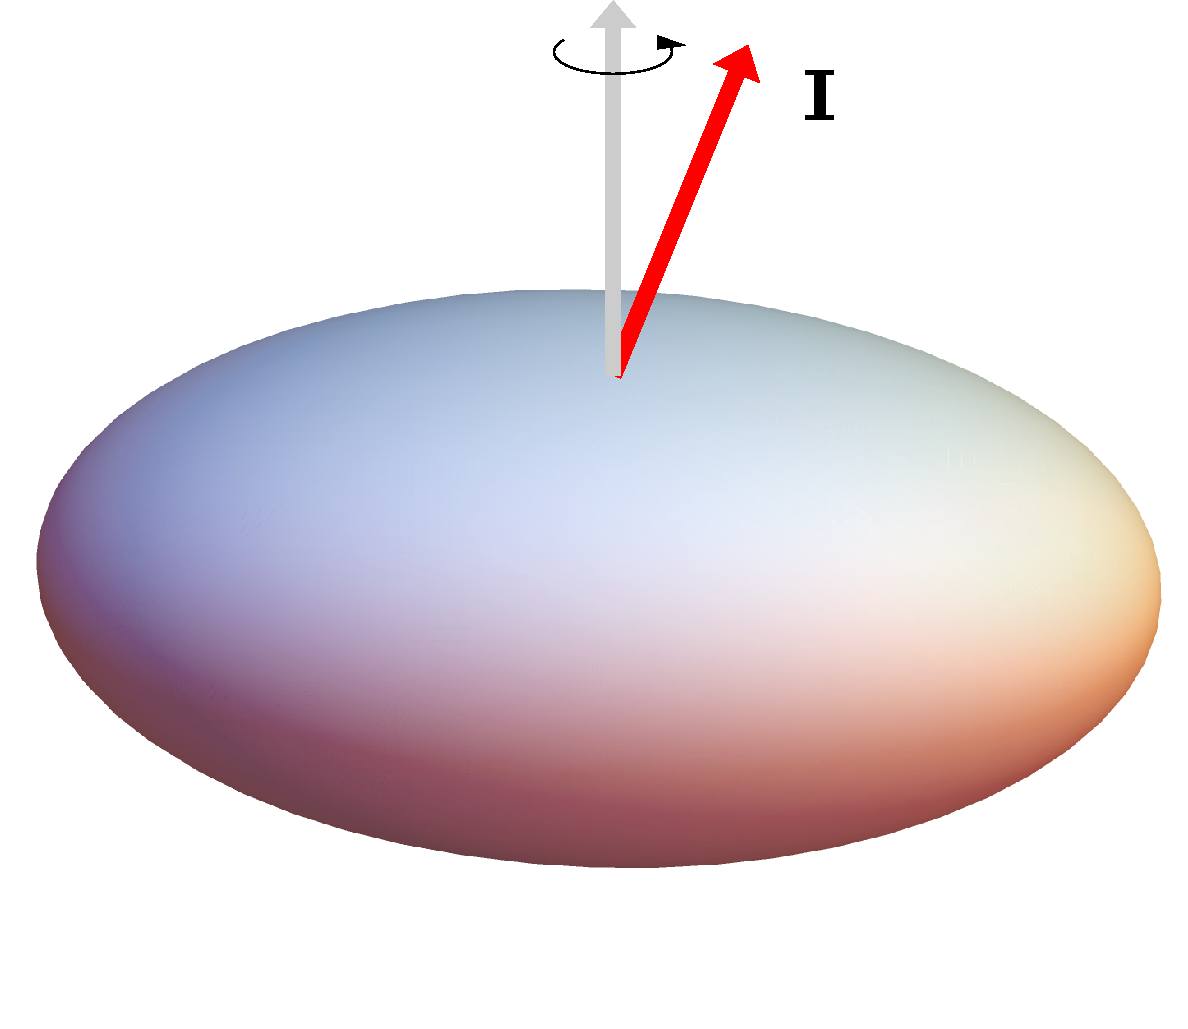
\includegraphics[scale=0.18]{Figs/triaxial-shapes-rotor-core.pdf}
  \end{figure}
\end{frame}

\begin{frame}
  \frametitle{Wobbling Spectrum}
\begin{block}{Even-$A$ Nuclei}
  \begin{itemize}
    \item Employing the Harmonic Approximation \textit{(Bohr, 1969)}
    \item $\hat{H}$ composed of a {\color{red}\emph{rotational}} part and {\color{blue}\emph{harmonic oscillation}} (i.e., wobbling) part:
  \end{itemize}
  \begin{align}
    \hat{H}={\color{red}\frac{\hbar^2}{2\mathcal{J}_\text{max}}I(I+1)}+{\color{blue}\hbar\omega_\text{wob}\left(n_w+\frac{1}{2}\right)}\ , n_w=0,1,2,\dots
    \label{wobbling-hamiltonian-even-A}
  \end{align}
\end{block}
\begin{figure}
  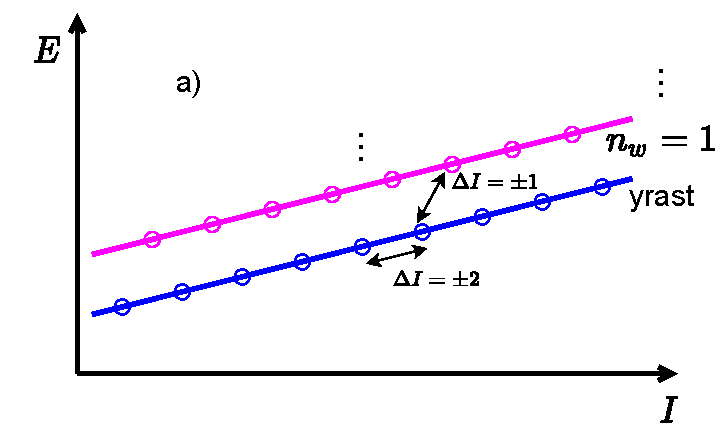
\includegraphics[scale=0.5]{Figs/wobbling_n_schematic-1.pdf}
  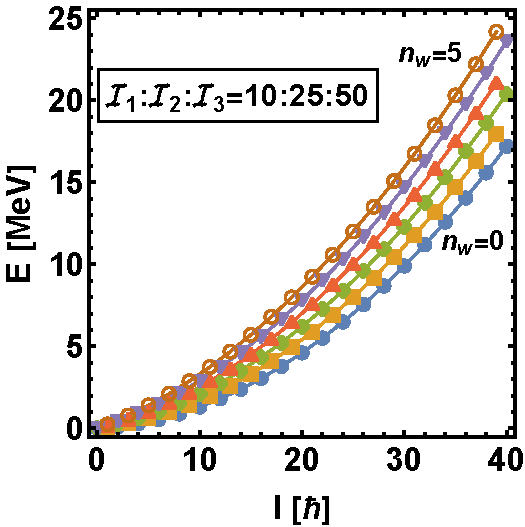
\includegraphics[scale=0.4]{Figs/wobblingFreq-evenA.pdf}
\end{figure}
\end{frame}

\begin{frame}
  \frametitle{}
  \begin{itemize}
    \item New experimental measurements show \emph{potential} wobbling candidates in the $A\approx 130$ region
    \item Three even-$A$ are studied with the \emph{simple wobbler} formalism
    \begin{enumerate}
      \item $^{130}$Ba
      \item $^{134}$Ce
      \item $^{136}$Nd
    \end{enumerate}
    \item Study the excited spectra: \emph{theoretical model checks the data?}
  \end{itemize}
\end{frame}

\begin{frame}
  \frametitle{New Results for A=130}
  \begin{minipage}{.8\textwidth}
    \begin{block}{Recent findings for even-even nuclei}
      \begin{itemize}
        \item Two wobbling bands have been identified experimentally in \textbf{$^\mathbf{130}$Ba} (\textit{Petrache et al., 2019})
        \item DFT+PRM description of the wobbling motion described the excited spectra (\textit{Chen et al., 2019})
        \item Stable triaxiality for $\beta=0.24$ and $\gamma=21.5^\circ$
        % \item Infer spin-dependence for $\mathcal{J}_{1,2,3}$
      \end{itemize}
    \end{block}
  \end{minipage}%
  \begin{minipage}{.2\textwidth}
    \begin{figure}
      \centering
      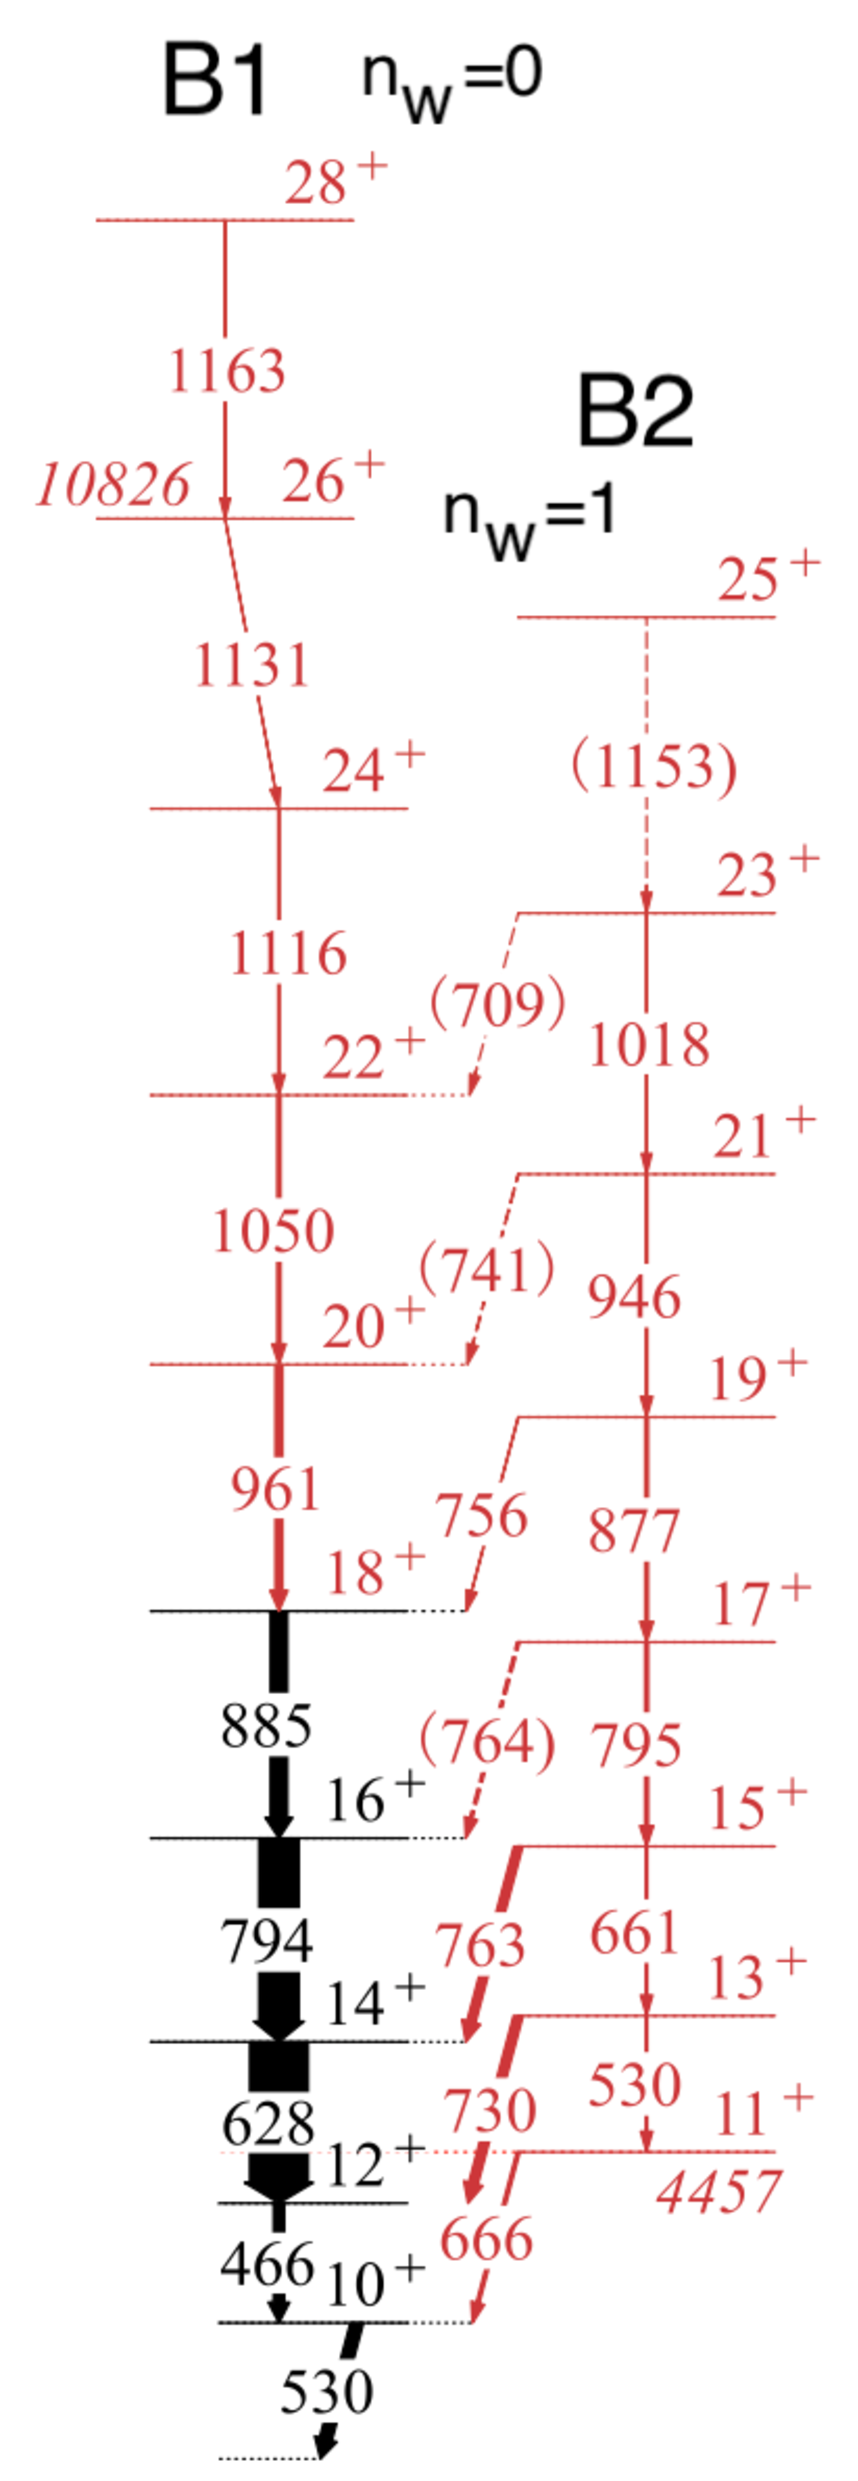
\includegraphics[scale=0.13]{Figs/ba-130-level-scheme.pdf}
      \tiny{\textit{Figure from Petrache et al., 2019}}
    \end{figure}
  \end{minipage}
\end{frame}



%---------------------------------------------------------
\end{document}
%---------------------------------------------------------

